\documentclass[a4paper, 10pt]{article}
\usepackage[utf8]{inputenc}
\usepackage{verbatim}
\usepackage{listings}
\usepackage{graphicx}
\usepackage{a4wide}
\usepackage{color}
\usepackage{amsmath}
\usepackage{amssymb}
\usepackage[dvips]{epsfig}
\usepackage[toc,page]{appendix}
\usepackage[T1]{fontenc}
\usepackage{cite} % [2,3,4] --> [2--4]
\usepackage{shadow}
\usepackage{hyperref}
\usepackage{titling}
\usepackage{marvosym }
\usepackage{subcaption}
\usepackage[noabbrev]{cleveref}

\usepackage{tikz}
\usetikzlibrary{arrows}

\renewcommand{\topfraction}{.85}
\renewcommand{\bottomfraction}{.7}
\renewcommand{\textfraction}{.15}
\renewcommand{\floatpagefraction}{.66}
\renewcommand{\dbltopfraction}{.66}
\renewcommand{\dblfloatpagefraction}{.66}
\setcounter{topnumber}{9}
\setcounter{bottomnumber}{9}
\setcounter{totalnumber}{20}
\setcounter{dbltopnumber}{9}


\setlength{\droptitle}{-10em}   % This is your set screw

\setcounter{tocdepth}{2}

\lstset{language=c++}
\lstset{alsolanguage=[90]Fortran}
\lstset{basicstyle=\small}
\lstset{backgroundcolor=\color{white}}
\lstset{frame=single}
\lstset{stringstyle=\ttfamily}
\lstset{keywordstyle=\color{red}\bfseries}
\lstset{commentstyle=\itshape\color{blue}}
\lstset{showspaces=false}
\lstset{showstringspaces=false}
\lstset{showtabs=false}
\lstset{breaklines}
\title{FYS3150 - Project 4}
\author{Gunnar Lange}
\begin{document}
\maketitle
\begin{abstract}
HEI
\end{abstract}
\tableofcontents
\section{Introduction}
The Ising model is a simple but very popular model for modelling phase transitions (see e.g. \textbf{HERE}). The model consists of a lattice of atomic spins which can have one of two possible values ("up" or "down"). The energy of each spin in their configuration is determined solely by their nearest neighbors. This model is widely used in statistical physics, in particular to study ferromagnetic phenomena.\\
\linebreak
We will investigate how multiple interesting thermodynamic quantities, including heat capacity, magnetic susceptibility, mean magnetization and mean energy, behave over time in the Ising model. We will investigate both ordered and disordered initial states of the lattice, checking the equilibration time in each case. Finally, we will also investigate phase transitions in the Ising model. We implement periodic boundary conditions and simulate temporal progression in the lattice by means of the Metropolis algorithm.\\
\linebreak
We begin with a discussion of the thermodynamic quantities that we will study, and how they are manifested in the Ising model. We then briefly discuss our chosen boundary conditions. Subsequently, we present the theory of phase transitions and the Metropolis algorithm, and discuss how we could identify the equilibrium of our system. We then discuss some technicalities relating to our implementation of the physical model, before presenting and discussing our results..
\section{Theoretical model}
\subsection{Thermodynamic quantities and the Ising model}
We study a square lattice consisting of $N\times N$ magnetic dipole moments (atomic spins) that can be in one of two states (+1 or -1). We wish to study how energy, magnetization, heat capacity and magnetic susceptibility develop in this system. This system, the Ising model, is a microcanonical system, i.e. we keep the temperature fixed. Then it is known from basic thermodynamics that this system can be described by Boltzmann statistics, i.e. by a distribution function given by:
\begin{equation}\label{eq:Boltzmann_probability}
P(E)=\frac{1}{Z}e^{-\frac{E}{k_BT}}
\end{equation}
Where $E$ is the energy of a microstate, $k_B$ is Boltzmann's constant and $T$ is the temperature of the system. We define $\beta = 1/(k_BT)$. Then $Z$, the partition function, is a normalization constant defined by:
\begin{equation}\label{eq:Parition_function}
Z=\sum_{i} e^{-\beta E_i}
\end{equation}
Where the sum is over all microstates, $i$. As $P(E)$ is a probability function, it may be used to define moments of a quantity $X$ according to the general scheme: 
\begin{equation}
\langle X^n \rangle = \frac{1}{Z}\sum_i X_i^n e^{-\beta E_i}
\end{equation}
Where $X_i$ is a quantity associated with the microstate $i$. This will be useful later, when computing the heat capacity and the magnetic susceptibility.\\
\linebreak
From this probability distribution, and the partition function, we can compute all thermodynamic quantities of interest.
\linebreak
In the simplest model of the Ising system, the energy is given by:
\begin{equation}\label{eq:ising_system_energy}
E=-J\sum_{\langle kl \rangle} s_ks_l
\end{equation}
Where the sum is over all the nearest neighbors in the lattice. $J$ is a constant which is determined by the quantum mechanical details of the system. We will simply set it to 1. The magnetization, on the other hand, is given as:
\begin{equation}
\mathcal{M}=\sum_i s_i
\end{equation}
Where the sum goes over all spins, $i$.\\
\linebreak
It is shown \textbf{here} that this  gives the following relation for thermodynamical quantities:\\
\textbf{Heat capacity}, $C_V$\\
\begin{equation}\label{eq:heat_capacity}
C_V=\frac{\langle E^2\rangle - \langle E \rangle^2}{k_BT^2}
\end{equation}
\textbf{Magnetic susceptibility}, $\chi$:
\begin{equation}\label{eq:magnetic_susp}
\chi=\frac{\langle \mathcal{M}^2\rangle - \langle \mathcal{M} \rangle^2}{k_BT}
\end{equation}
The first moment of the energy, $\langle E \rangle$, can also be computed in another way, which will be useful later, namely:
\begin{equation}
\langle E \rangle = -\frac{\partial \ln Z}{\partial \beta}
\end{equation}
This is proved \textbf{here}.
\subsection{Periodic boundary condition}
From the above description, it is not obvious how to treat the boundaries of the lattice. We will assume the  lattice (representing for example a crystalline structure in a solid) to be essentially infinite in all directions. In this case, we can assume the boundary to have no effect on the behavior of our crystal. Therefore, we let our crystal "loop around" itself, that is, we let neighbor of the leftmost crystals be the rightmost crystals, simulating a "continuation"of the crystals to the left. We adapt the same approach for the other edges of the crystals.

\subsection{Phase transitions in the Ising model}\label{phase_tranisition}
It is well known from literature \textbf{REFERENCE} that there exists a critical temperature, $T_C$, at which phase transitions can be observed in the Ising model. At this temperature, one can observe spikes in the thermodynamic quantities. Near $T_C$,our thermodynamic quantities can be modelled as simple power laws. As shown \textbf{HERE}, these laws take the following forms:
\begin{equation}\label{eq:analytical_thermo_near_critical}
\begin{split}
\langle \mathcal{M}(T)\rangle \sim (T-T_C)^{\beta}\\
C_V(T) \sim |T_c-T|^{-\gamma}\\
\mathcal{X}(T) \sim |T_C-T|^{-\alpha}
\end{split}
\end{equation}
Where $\alpha, \beta$ and $\gamma$ are critical exponents, given by: $\alpha=0,\  \beta=1/8,\ \gamma=7/4$\\
\linebreak
The temperature $T_C$ will depend upon the number of spins in our lattice, $N$. Ideally, the number of spins should be close to infinite. However, our computational capacities limit us to systems with a maximum size of about $N=140$. Luckily, however, we can estimate the critical temperature for $N=\infty$, $T_C(N=\infty)$ from the critical temperature at a finite $N$, $T_C(N)$ by the equation shown \textbf{HERE}, which we reproduce:
\begin{equation}\label{eq:Critical_temp_at_infinite}
T_C(N)-T_C(N=\infty)=aN^{-1/\nu}
\end{equation}
Where $a$ is a constant, which can be determined from:
\begin{equation}\label{eq:a:equation}
a=\frac{T_C(N_1)-T_C(N_2)}{N_1^{-1/\nu}-N_2^{-1/\nu}}
\end{equation}
$\nu$ is another critical temperature, which has the exact result $\nu=1$. Thus we can estimate the critical temperature by computing a from equation \ref{eq:a:equation} for two different lattice sizes, $N_1$ and $N_2$, and then solving equation \ref{eq:Critical_temp_at_infinite} for $T_C(N=\infty)$. Note that we can also use the equations in \ref{eq:analytical_thermo_near_critical} near the critical temperature as analytic solutions to which we can compare our numerical results. 
\subsection{The Metropolis Algorithm}\label{Monte-Carlo_algo}
We will use Monte-Carlo simulations to model the time development of our spin system. Assume that we have an initial random configuration of spins, with energy $E_b$ (which we have calculated from equation \ref{eq:ising_system_energy}). We employ the famous Metropolis algorithm to achieve this. The Metropolis algorithm is described in detail \textbf{HERE}, but it can be briefly summarized in the following steps:
\begin{itemize}
\item Randomly select $N^2$ spins from the $N\times N$ lattice.
\item For each spin, calculate the change in energy, $\Delta E$, that the system would experience if we were to flip it
\item Draw a random number, $\zeta$ uniformly between $0$ and $1$, and compare it to $e^{-\beta \Delta E}$. \item If $\zeta \leq e^{-\beta \Delta E}$, flip the spin, else do not flip the spin (note that any spin flip with $\Delta E < 0$ will always be performed).
\item Update the thermodynamic quantities.
\end{itemize}
It can be shown (\textbf{REFERENCE}) that this simple scheme will evolve the system towards its equilibrium state (dictated by the Helmoltz free energy). Thus, repeating the above steps many times, which corresponds to performing many Monte-Carlo cycles, will evolve our system towards equilibrium. We will therefore use the number of Monte-Carlo cycles synonymously with time in our simulation.
\subsection{Equilibrium of the system}\label{equilibrium_system}
We choose multiple different starting configurations of our lattice, including a homogeneous configuration (all spins initially point the same way), and a random configuration (spins drawn from a uniform distribution). We expect that our system should approach a stationary state after some time, $T$. There are multiple indicators of this state. First of all, we expect the number of accepted spins to reach a low, constant value, i.e. the total number of accepted spins  per time steadily decreasing curve, approaching an equilibrium value. Most spins will be in their stable configuration at equilibrium, and therefore few flips will be occur. We also expect all thermodynamical quantities to reach an equilibrium state, where the variations are small. Both of these will be good indicators for equilibrium. 
\subsection{Analytic solution for the 2x2 case with periodic boundary conditions}\label{2x2analytic}
It is not too difficult to find an analytic solution for a small latice consisting only of $2\times 2$ spins. This analytic solution provides an important consistency check for our algorithm. Assume therefore that we have a lattice consisting of 4 magnetic dipole moments, labelled as shown in figure \ref{fig:2x2spins}:
\begin{figure}[!ht]
\centering
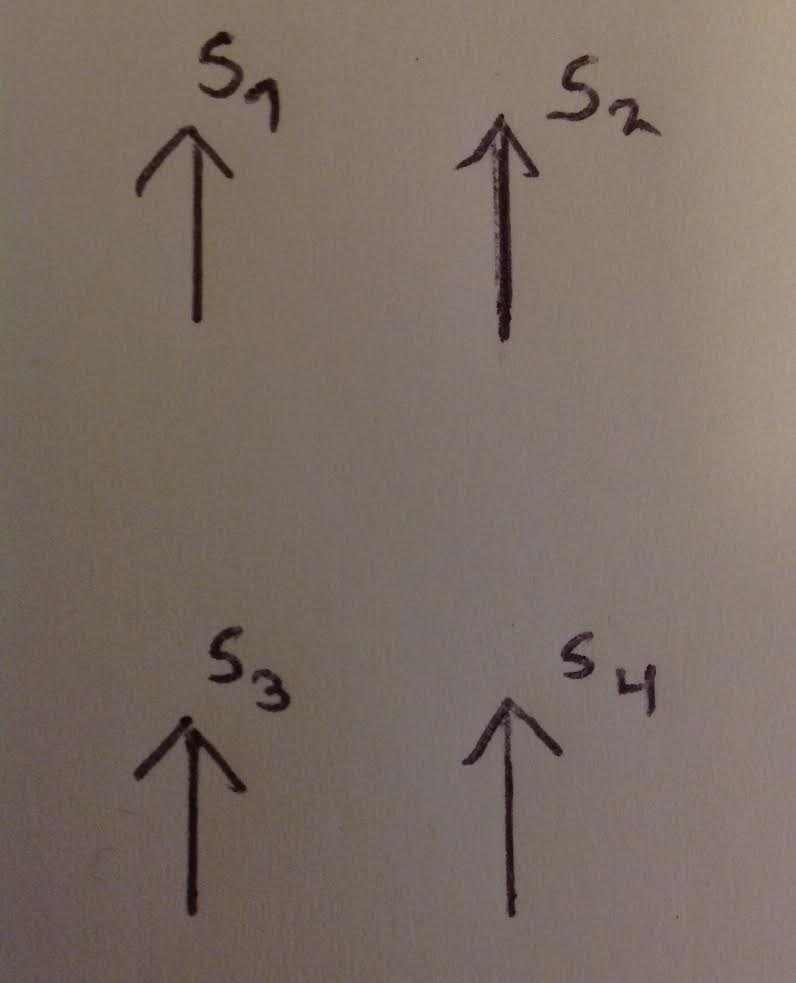
\includegraphics[scale=0.2]{SpinSystem.jpeg}
\caption{One microstate of our $2 \times 2$ lattice, illustrating how we label the spins.}\label{fig:2x2spins}
\end{figure}
\newpage
We notice first there are only 5 distinct macrostates, namely 0 to 4 spins up. There should be a total of $2^4=16$ microstates. It is clear that the extremes (0 spins up and 4 spins up),  have only one microstate associated with them. The states 1 spin up and 3 spins up each have 4 associated microstates (you can flip one of the four spins). This implies that there are a total of 6 ways to have the state 2 up and 2 down. This is summarized in the table below:\\
\begin{center}
\begin{tabular}{|c|c|}
\hline
Spins up & Number of microstates\\
\hline
4 & 1\\
3 & 4\\
2 & 6\\
1 & 4\\
0 & 1\\
\hline
\end{tabular}
\end{center}
Now we must investigate the energy of each of these states. In general, the energy with periodic boundary condition for a $2\times 2$ lattice can be written as:
$$E=-J\left[s_1s_2+s_2s_1+s_1s_3+s_3s_1+s_2s_4+s_4s_2+s_3s_4+s_4s_3\right]$$
From this it follows immediately that the energy for the states for 4 spins up or 4 spins down is $-8J$. If we flip one spin, we will flip the sign of exactly half the terms (because each spin occurs in four of the eight pairs). Thus the energy will be zero. If we flip two spins, we can either flip spins that are nearest neighbors (such as $s_1$ and $s_2$, $s_1$ and $s_3$, $s_2$ and $s_4$ or $s_3$ and $s_4$), or we can flip spins that are not nearest neighbors (such as $s_1$ and $s_4$ or $s_2$ and $s_3$). In the first case, we flip the sign of four of the terms in the sum (namely all those that contain one of the two  spins we flip). Thus the total energy will be zero. In the other case, we flip the sign of all terms. Thus the total energy will be 8J.\\
\linebreak
To find the magnetization, we must simply sum the total number of spin up and subtract the number of spin down. This is all summarized in the table below:
\begin{center}
\begin{tabular}{|c|c|c|c|}
\hline
Spins up &  Energy [J]& Magnetization[J/T] &Number of microstates\\
\hline
4 &-8J&4&1\\
3 &0 & 2 & 4\\
2 &0 &0 & 4\\
2 & 8J & 0 &2\\
1 &0&-2 & 4\\
0 & -8J & -4& 1\\
\hline
\end{tabular}
\end{center}
This enables us to calculate the partition function as:
$$Z=\sum_{i=1}^{16} e^{-\beta E_i}$$
Where $\beta=1/k_BT$. As most of the energies are zero, this is relatively straightforward and gives:
$$Z=2e^{8\beta J}+2e^{-8\beta J} + 12=4\cosh (8J\beta) +12$$
We can now compute the expected value of the energy as:
\begin{equation}\label{eq:2x2energy}
\langle E \rangle =  -\frac{\partial \ln Z}{\beta}=-\frac{\partial}{\partial \beta}\ln\left(2e^{8\beta J}+2e^{-8\beta J}+12\right)=\frac{-16Je^{8\beta J}+16Je^{-8\beta J}}{2e^{8\beta J}+2e^{-8\beta J}+12}=-\frac{8J\sinh(8\beta J)}{\cosh(8\beta J)+3}
\end{equation}
Similarly, we can compute the heat capacity, $C_V$, as:
$$C_V=\frac{d\langle E \rangle}{dT}=\frac{d}{dT}\left(\frac{-16Je^{\frac{8J}{k_BT}}+16Je^{-\frac{8J}{k_BT}}}{2e^{\frac{8J}{k_BT}}+2e^{-\frac{8J}{k_BT}}+12}\right)$$
However, this is an ugly differentiation. Therefore, we will instead use the relation:
$$C_V=\frac{\langle E^2 \rangle - \langle E \rangle^2}{k_BT^2}$$
The square of the expected value of the energy is given by:
$$\langle E^2\rangle=\frac{1}{Z} \sum_{i=1}^ {16}E_i^2e^{-\beta E_i}$$
The sum is easy to compute:
$$\sum_{i=1}^{16}E_i^2e^{-\beta E_i}=64J^2e^{8J\beta}+128J^2e^{-8J\beta}+64J^2e^{8J\beta}=128J^2\left(e^{8J\beta}+e^{-8J\beta}\right)$$
Which gives:
$$\langle E^2\rangle = \frac{128J^2\left(e^{8J\beta}+e^{-8J\beta}\right)}{2e^{8J\beta}+2e^{-8J\beta}+12}=\frac{256J^2\cosh(8J\beta)}{4\cosh(8J\beta)+12}$$
From which it follows that:
$$C_V=\frac{1}{k_BT^2}\left(\frac{128J^2\left(e^{8J\beta}+e^{-8J\beta}\right)}{2e^{8J\beta}+2e^{-8J\beta}+12}-\left(\frac{-16Je^{8\beta J}+16Je^{-8\beta J}}{2e^{8\beta J}+2e^{-8\beta J}+12}\right)^2\right)$$

\begin{equation}\label{eq:2x2Cv}
C_V=\frac{1}{k_BT}\left(\frac{256J^2\cosh(8J\beta)}{4\cosh(8J\beta)+12}-\left(\frac{-8J\sinh(8J\beta)}{\cosh(8J\beta)+3}\right)^2\right)
\end{equation}

Magnetization can be computed as:
$$\langle M \rangle=\frac{1}{Z}\sum_{i=1}^{16}M_ie^{-\beta E_i}$$
The sum can be computed as:
$$\sum_{i=1}^{16}M_ie^{-\beta E_i}=4e^{8J\beta}+8-8-4e^{8J\beta}=0$$
Thus the expected value of the magnetization is zero. The expected value of the absolute value of the magnetization on the other hand is:
\begin{equation}\label{eq:2x2abs_mag}
\langle |M|\rangle =\frac{1}{Z}\sum_{i=1}^{16}|M_i|e^{-\beta E_i}=\frac{1}{Z}\left( 4e^{8J\beta}+4\cdot 2+ 4\cdot 2 +4e^{8J\beta}\right)=\frac{2e^{8J\beta}+4}{\cosh(8J\beta)+3}
\end{equation}
The square of expected value of the magnetization can be computed as:
$$\langle M^2 \rangle = \frac{1}{Z}\sum_{i=1}^{16}M_i^2e^{-\beta E_i}=\frac{1}{Z}\left(16e^{8\beta J}+4\cdot 4+4\cdot 4+16e^{8\beta J}\right)=\frac{8e^{8\beta J}+8}{\cosh(8J\beta)+3}$$
Now it is easy to compute the susceptibility:
\begin{equation}\label{eq:2x2Sus}
\chi = \frac{\langle M^2\rangle - \langle M \rangle^2}{k_BT}=\frac{1}{k_BT}\left(\frac{8e^{8\beta J}+8}{\cosh(8\beta J)+3}\right)
\end{equation}
We can now simulate a $2\times 2$ lattice, and check if equations \ref{eq:2x2energy}, \ref{eq:2x2Cv}, \ref{eq:2x2abs_mag} and \ref{eq:2x2Sus} hold true, which gives us a consistency check for our methods.
\section{Methods}
\subsection{Energy in our system}\label{energy_in_system}
Note that the sum in equation \ref{eq:ising_system_energy} is only over the nearest neighbors. Therefore, the change in energy from the flip of a single spin (as in the Metropolis algorithm), depends only on the configuration of the nearest neighbors (which are only four spins). This means that there are only a limited number of possible energy differences, $\Delta E$. As shown \textbf{HERE}, the only possible values of $\Delta E$ are:
$$\Delta E = \{ -8J, -4J, 0, 4J, 8J\}$$
Wen can therefore precompute the Boltzmann factor, $e^{-\beta \Delta E}$, for all of these possible flips. Thus, for each spin flip in the Metropolis algorithm, we can simply check the configuration of the neighboring spins, and then assign an energy change, $\Delta E$, by checking the state of the neighboring spins, as described in more detial in section \ref{metropolis_algo_implementation}.\\
\linebreak
Not that this works well for all but the initial configuration. For the initial configuration, we will have to compute the total energy. This can be done by a nested for-loop construction, where we always include the energy from the spin above and to the left of our current spin, to avoid double counting. This is shown in the pseudo code below:
\lstinputlisting{Pseudo_code_total_energy.cpp}
\subsection{Implementing periodic boundary conditions}
The periodic boundary conditions can be implemented by using modular division. Each spin will have four nearest neighbors in the lattice. Assume our selected spin is at $x_i$, $y_i$. This spin will be affected by the spin at position $x_{i+1}$, $y_i$ and $x_{i-1}$, $y_i$ (as well as the corresponding spins in the y-idrection). If $x_i$ is on the boundary of our lattice, however, the point to the left or to the right may not exist. Therefore, we find adjacent points by using the following formula:
\begin{equation}\label{eq:modular_arithmetic}
x_{i+1}=(x_{i+1}+N) \bmod N
\end{equation}
Note that, if $x_{i+1}$ happens to element number $N$, this equation gives element 0, and if $x{i-1}$ happens to be element 0, the equation gives element number $N-1$. Thus, this implements the periodic boundary conditions.
\subsection{Implementing the Metropolis algorithm}\label{metropolis_algo_implementation}
The Metropolis algorithm is also implemented as two nested for-loops: the outer one, where we sum over Monte Carlo steps, and the inner one where we sum over $N\times N$ randomly selected spins.\\
\linebreak
As we mentioned in section \ref{energy_in_system}, we can precompute all possible energy differences. Thus, when we propose a spin flip, we must simply compute the energy change due to the flip, which can be found from:
$$\Delta E = 2J\sum_k s_is_k$$
Where the sum extends over all neighbors of the spin $s_i$. We can then associate this $\Delta E$ with the correct, precomputed, Boltzmann factor, and do the comparison described in section \ref{Monte-Carlo_algo}.  This is shown in Pseudo-code below. Note that we here disregard the periodic boundary conditions, for improved readability. 
\lstinputlisting{Pseudo_code_Metropolis.cpp}
\subsection{Investigating the time taken to arrive at the most likely state and the underlying probability distribution}
We wish to investigate how the equilibration time (time to reach most likely state) of our system depends on the temperature of our system, and on the initial configuration. We adapt a plain graphical approach - we simply plot the time development of the mean energy and the mean absolute value of the magnetization, to find when the (initially large) deviations die out. An alternative way to characterize equilibrium is, as discussed in section \ref{equilibrium_system}, with the total number of accepted configurations. Therefore, we include a plot of this as well.\\
\linebreak
Additionally, we would also like to characterize the probability distribution governing the equilibrium state. Therefore, we start our simulation after the time which we determined to be the equilibration time, and compute the number of times a given energy $E$ appears.
\subsection{Investigating phase transitions}
To investigate the phase transitions that occur in the Ising system, we employ the fact that the analytic result for $T_C(N=\infty)$ from section \ref{phase_tranisition} is approximately 2.269 \textbf{REFERENCE}. Thus we choose temperatures close to this, and find the critical temperature (the temperature at which a divergent behavior is observed for the heat capacity and the magnetic susceptibility). Then we compare with the equations from section \ref{phase_tranisition}.
\subsection{Parallelizing our code}
Note that the quantities that we are investigating are statistical measures such as the expected value or the variance. Increasing the number of cycles will therefore result in a better data. To maximize the number of cycles that we can obtain we parallelize our code, using MPI. Thus, we let all four cores on our computer run separate simulations, and then compute the means using the data from all of these runs.\footnote{Note that we initially intended to run on a larger cluster but, due to time constraints, this was not possible.}
\section{Results}
In this section, we present the results from our investigation. We postpone an extended discussion of these results until the next section.
\subsection{Results from the 2 $\times$ 2 lattice}
We begin by investigating the number of steps required to get a good correspondence between the analytic expressions from section \ref{2x2analytic} and our simulations. We choose to compare the heat capacity of the system, as this has the most complex form. We let each core run an $N$ that is divisible by $10$, so that the total number of steps will be $4$ times a number divisible by $10$. Note that we plot all of these quantities \textit{per spin} to ease readability.
\begin{figure}[!ht]
    \centering
    \begin{subfigure}[H!]{0.5\textwidth}
        \centering
        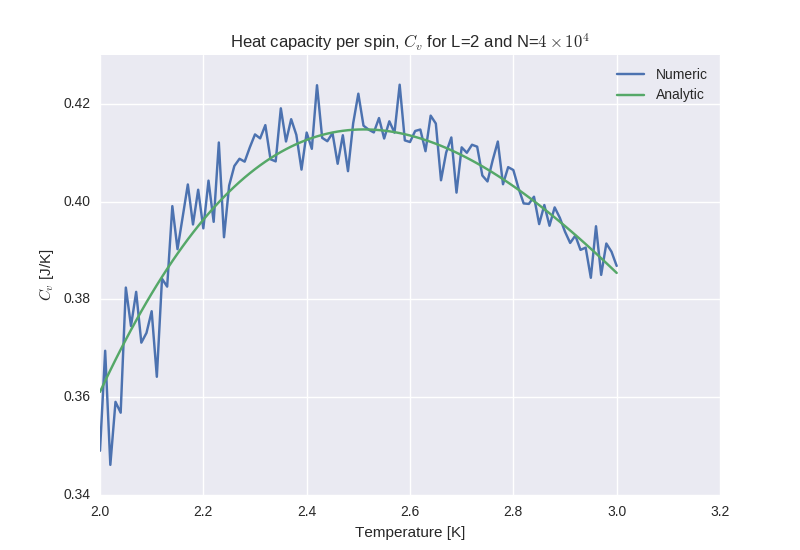
\includegraphics[height=2.2in]{L2Cv4e4.png}
        \caption{$N=4\times 10^4$}
    \end{subfigure}%
    ~ 
    \begin{subfigure}[H!]{0.5\textwidth}
        \centering
        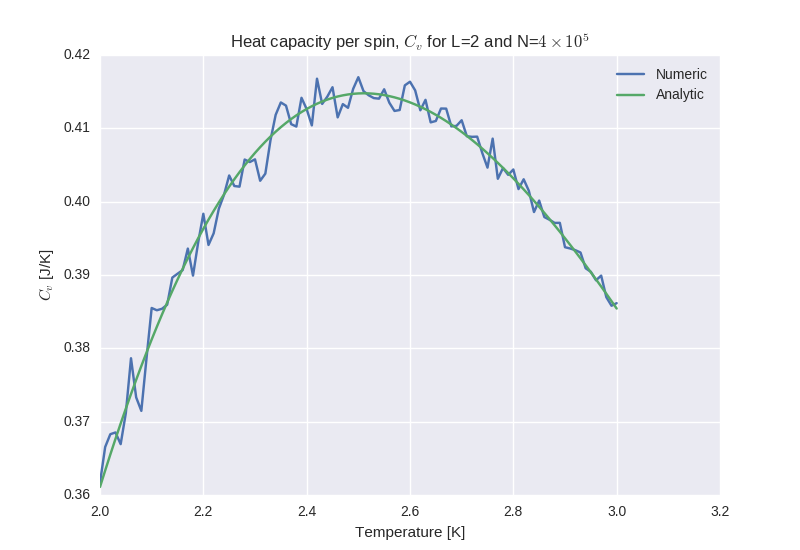
\includegraphics[height=2.2in]{L2Cv4e5.png}
        \caption{$N=4\times 10^5$}
    \end{subfigure}
    \begin{subfigure}[H!]{0.5\textwidth}
        \centering
        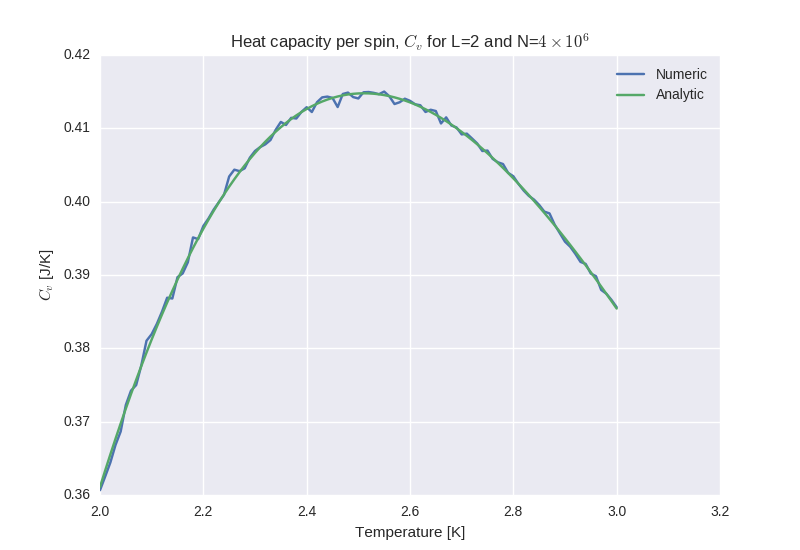
\includegraphics[height=2.2in]{L2Cv4e6.png}
        \caption{$N=4\times 10^6$}
    \end{subfigure}%
    ~ 
    \begin{subfigure}[H!]{0.5\textwidth}
        \centering
        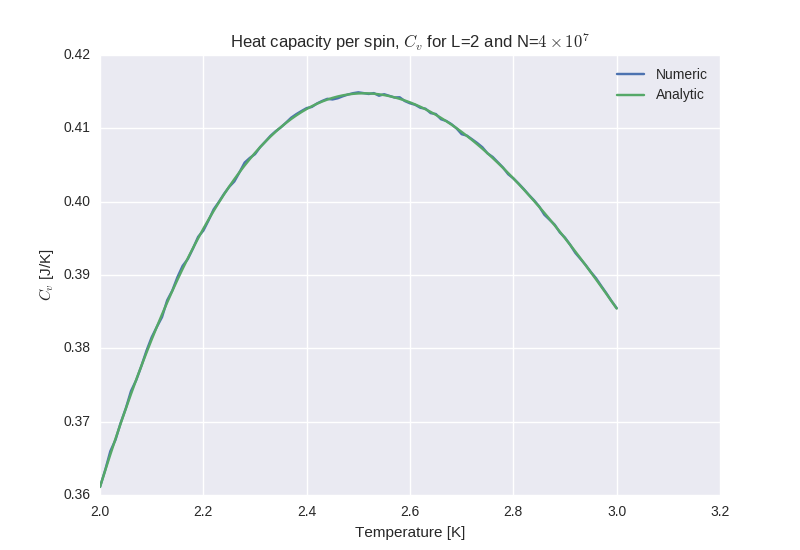
\includegraphics[height=2.2in]{L2Cv4e7.png}
        \caption{$N=4\times 10^7$}
    \end{subfigure}
    \caption{Comparison of the numeric and analytic solution of heat capacity and mean energy per spin for the $2\times 2$ lattice. We plot multiple Monte Carlo steps, $N$, to find where the correspondence becomes good.}\label{fig:2x2_nsteps}
\end{figure}

Looking at the plots, we choose $N=4\times 10^7$ as the required $N$, as this gives an excellent correspondence between the analytic and the numeric solution. The plots of our thermodynamic quantities in the $2\times 2$ lattice for this value of $N$ are shown below:
\begin{figure}[!ht]
    \centering
    \begin{subfigure}[H!]{0.5\textwidth}
        \centering
        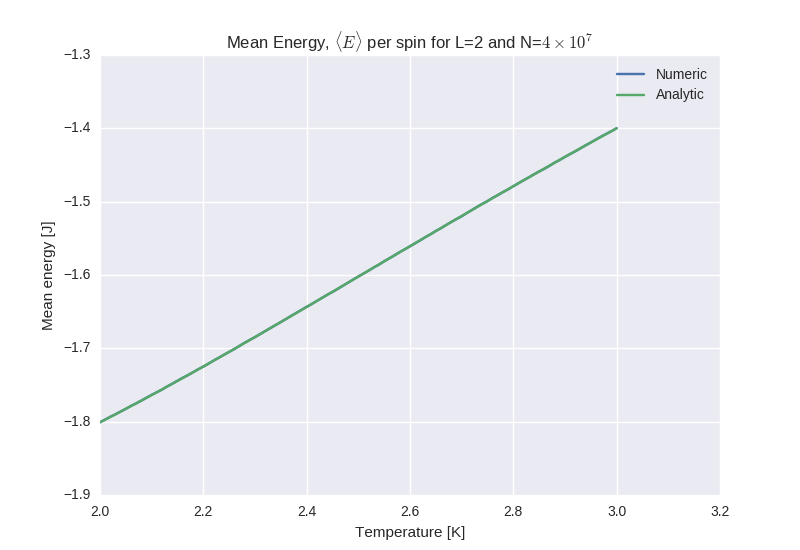
\includegraphics[height=2.2in]{L2MeanEner4e7.png}
        \caption{Mean energy per spin}
    \end{subfigure}%
    ~ 
    \begin{subfigure}[H!]{0.5\textwidth}
        \centering
        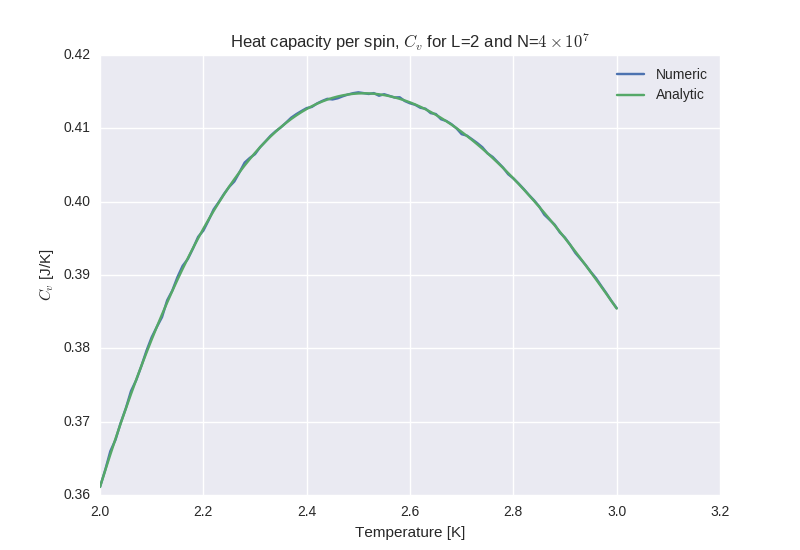
\includegraphics[height=2.2in]{L2Cv4e7.png}
        \caption{Heat capacity per spin}
    \end{subfigure}
    ~
     \begin{subfigure}[H!]{0.5\textwidth}
        \centering
        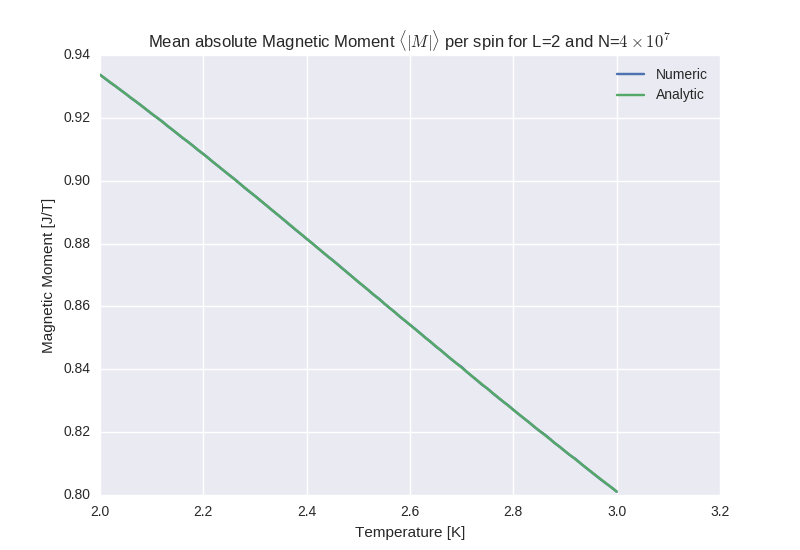
\includegraphics[height=2.2in]{L2MeanabsMag4e7.png}
        \caption{Mean absolute magnetic moment per spin}
    \end{subfigure}%
    ~ 
    \begin{subfigure}[H!]{0.5\textwidth}
        \centering
        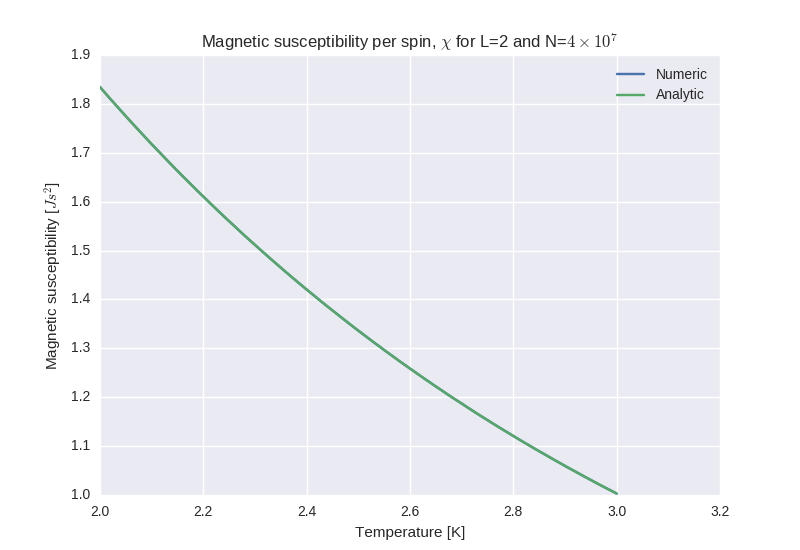
\includegraphics[height=2.2in]{L2MagSus4e7.png}
        \caption{Magnetic susceptibility per spin}
    \end{subfigure}
    \caption{Comparison of the numeric and  analytic solution for the mean energy per spin, heat capacity per spin, mean absolute magnetic moment per spin and magnetic susceptibility of the $2 \times 2$ lattice. }\label{fig:2x2_thermo}
\end{figure}
\subsection{Results from our investigation into the equilibration time}
We choose to use a larger lattice, of $20 \times 20$ spins, to investigate the time (measured in number of sweeps of the lattice) that it takes our system to achieve equilibrium. We investigate this first with a low temperature (letting $kT/J=1.0$). We investigate how this system develops if we start with an ordered initial state (all spins pointing up) and if we start with a disordered (uniformly distributed) state. A plot of the mean energy and the mean absolute value of the magnetization in this case is shown below:
\begin{figure}[!ht]
    \centering
    \begin{subfigure}[H!]{0.5\textwidth}
        \centering
        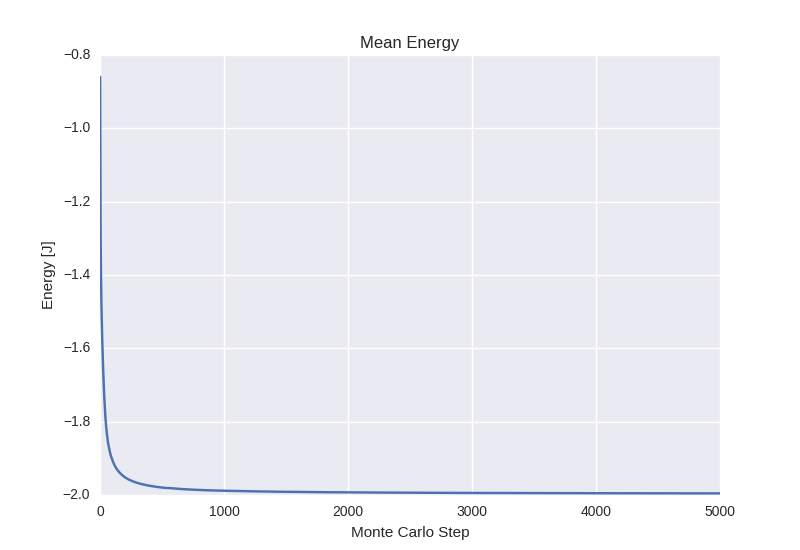
\includegraphics[height=2.2in]{meanEnergyWRandomStart.png}
        \caption{Mean energy per spin from disordered state}
    \end{subfigure}%
    ~ 
    \begin{subfigure}[H!]{0.5\textwidth}
        \centering
        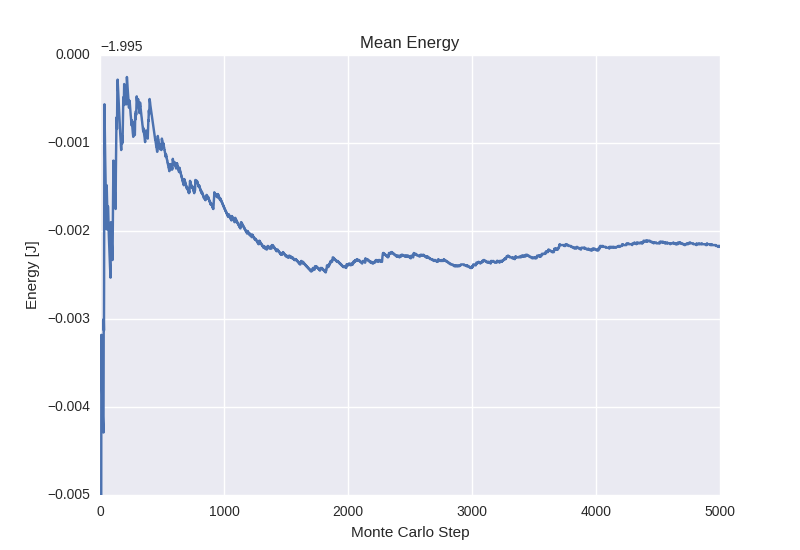
\includegraphics[height=2.2in]{meanEnergyWUpStart.png}
        \caption{Mean energy per spin from uniform state}
    \end{subfigure}
        ~
     \begin{subfigure}[H!]{0.5\textwidth}
        \centering
        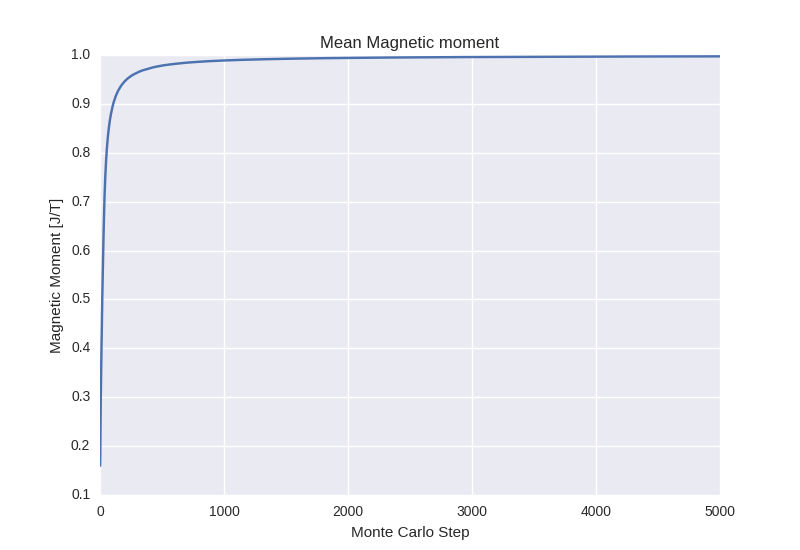
\includegraphics[height=2.2in]{meanMagMomWRandomStart.png}
        \caption{Mean absolute magnetic moment per spin from disordered state}
    \end{subfigure}%
    ~ 
    \begin{subfigure}[H!]{0.5\textwidth}
        \centering
        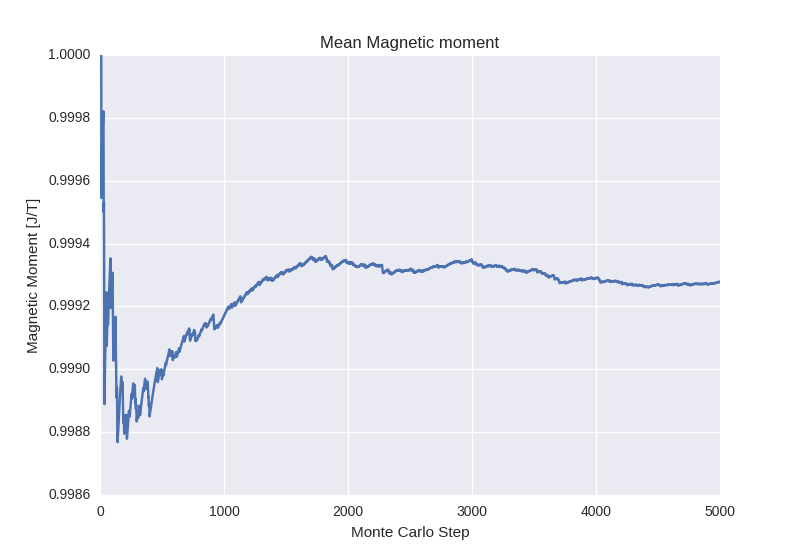
\includegraphics[height=2.2in]{meanMagMomWUpStart.png}
        \caption{Mean absolute magnetic moment per spin from uniform state}
    \end{subfigure}
      \caption{Time development of mean energy and mean magic moment per spin for two different initial configurations. This is at temperature $kT/J=1.0$.}\label{fig:20x20_Sweep_T_1}
\end{figure}
We also plot the same quantities for a temperature of $kT/J=2.4$ in the figure below:
\begin{figure}[!ht]
    \centering
    \begin{subfigure}[H!]{0.5\textwidth}
        \centering
        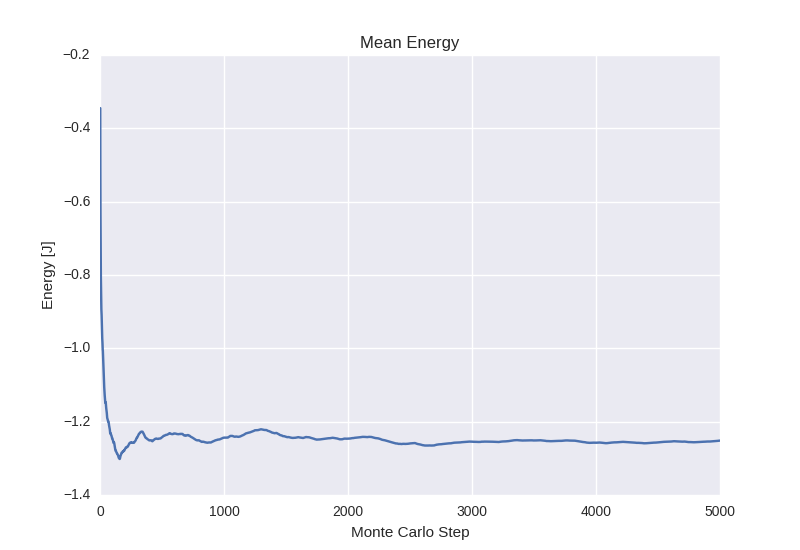
\includegraphics[height=2.2in]{meanEnergyWRandomStartT24.png}
        \caption{Mean energy per spin from disordered state}
    \end{subfigure}%
    ~ 
    \begin{subfigure}[H!]{0.5\textwidth}
        \centering
        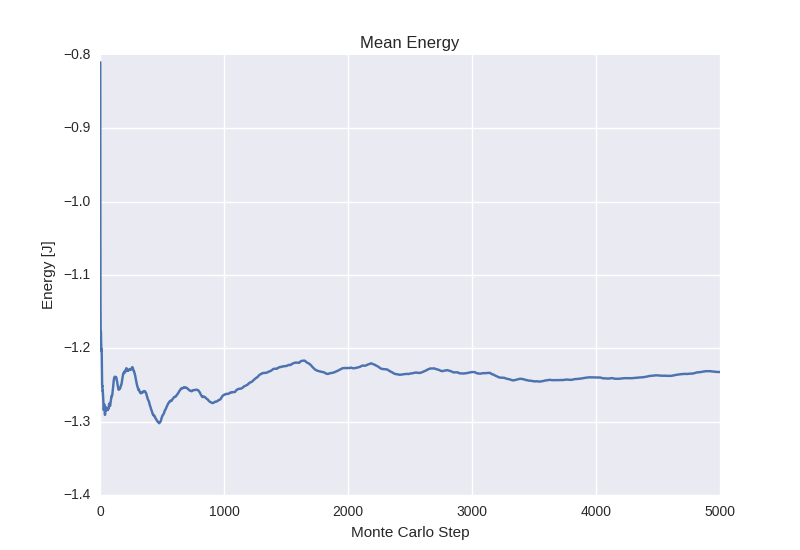
\includegraphics[height=2.2in]{meanEnergyWUpStartT24.png}
        \caption{Mean energy per spin from uniform state}
    \end{subfigure}
        ~
     \begin{subfigure}[H!]{0.5\textwidth}
        \centering
        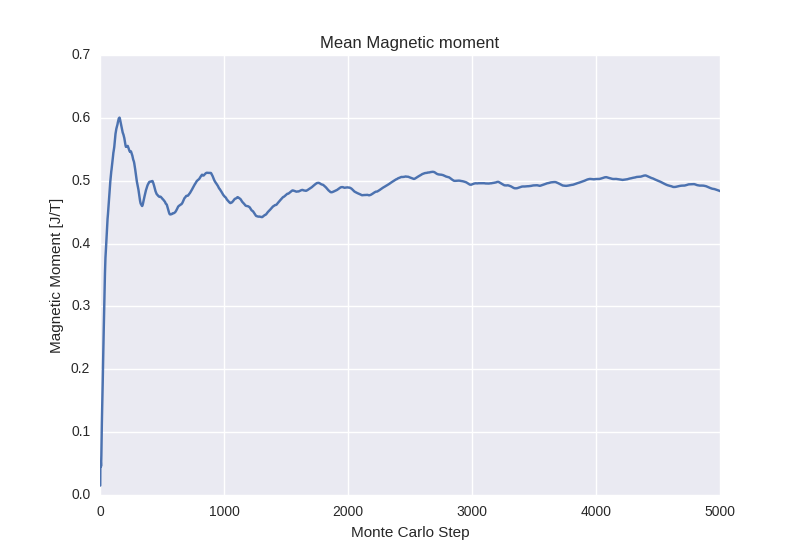
\includegraphics[height=2.2in]{meanMagMomWRandomStartT24.png}
        \caption{Mean absolute magnetic moment per spin from disordered state}
    \end{subfigure}%
    ~ 
    \begin{subfigure}[H!]{0.5\textwidth}
        \centering
        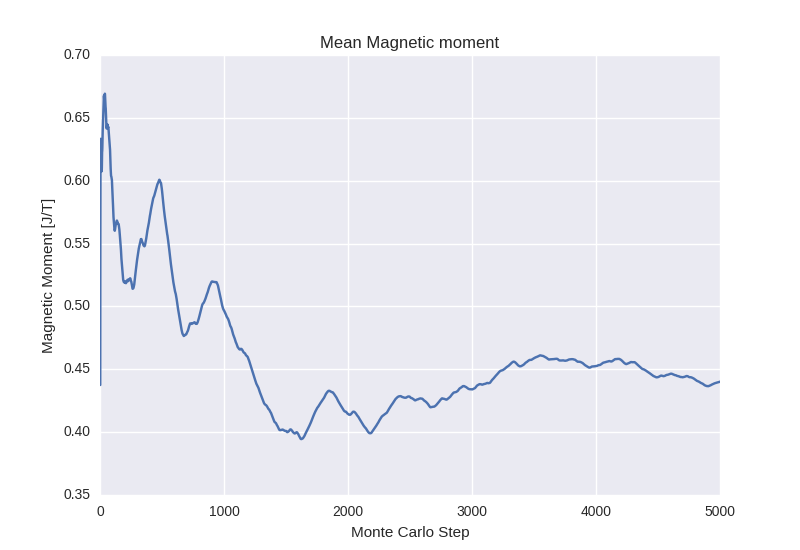
\includegraphics[height=2.2in]{meanMagMomWUpStartT24.png}
        \caption{Mean absolute magnetic moment per spin from uniform start}
    \end{subfigure}
      \caption{Time development of mean energy and mean magic moment per spin for two different initial configurations.}\label{fig:20x20_Sweep_T_24}
\end{figure}

Finally, we also plot the number of accepted flips per spin and time, to get a sense of how many spins the Metropolis algorithm flips at every time step. We do this for two different temperatures, again using both an ordered and a disordered state.
\begin{figure}[!ht]
    \centering
    \begin{subfigure}[H!]{0.5\textwidth}
        \centering
        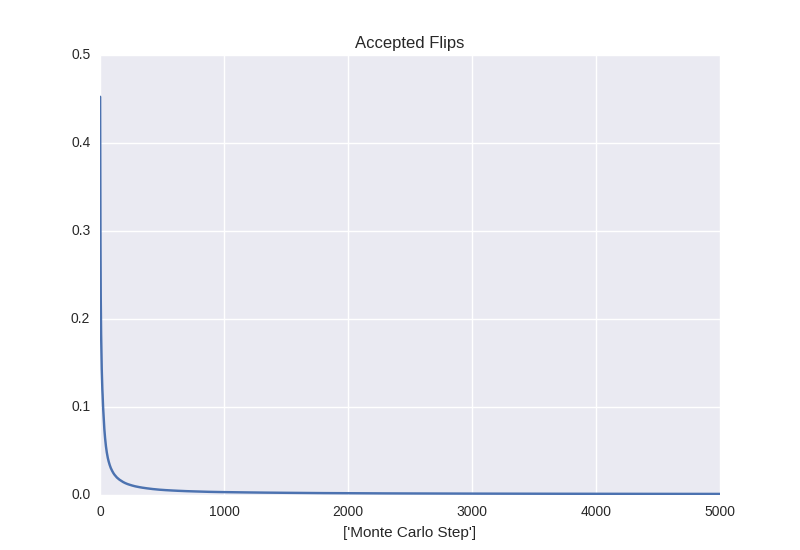
\includegraphics[height=2.2in]{flipsWRandomStart.png}
        \caption{Mean energy per spin from disordered state}
    \end{subfigure}%
    ~ 
    \begin{subfigure}[H!]{0.5\textwidth}
        \centering
        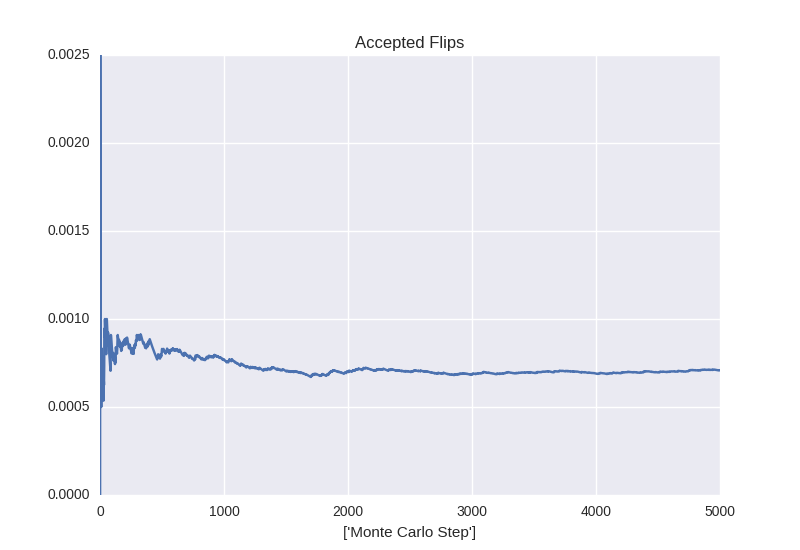
\includegraphics[height=2.2in]{flipsWUpStart.png}
        \caption{Mean energy per spin from uniform state}
    \end{subfigure}
        ~
     \begin{subfigure}[H!]{0.5\textwidth}
        \centering
        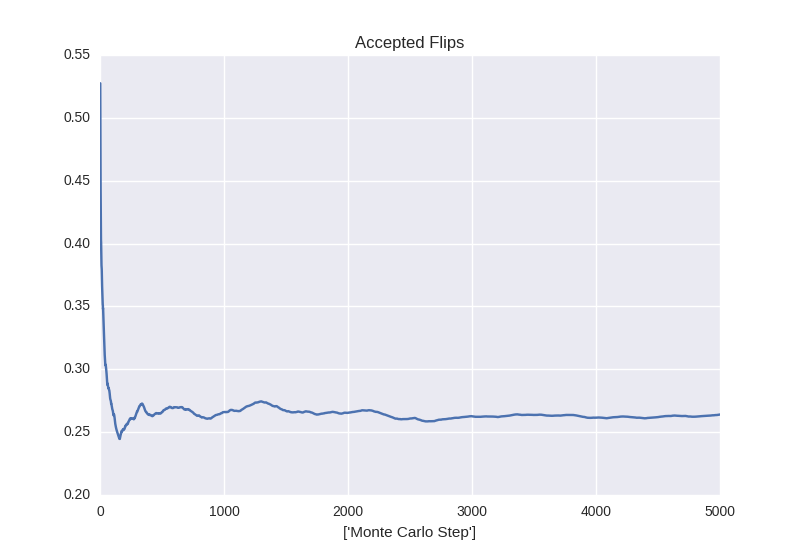
\includegraphics[height=2.2in]{flipsWRandomStartT24.png}
        \caption{Mean absolute magnetic moment per spin from disordered state}
    \end{subfigure}%
    ~ 
    \begin{subfigure}[H!]{0.5\textwidth}
        \centering
        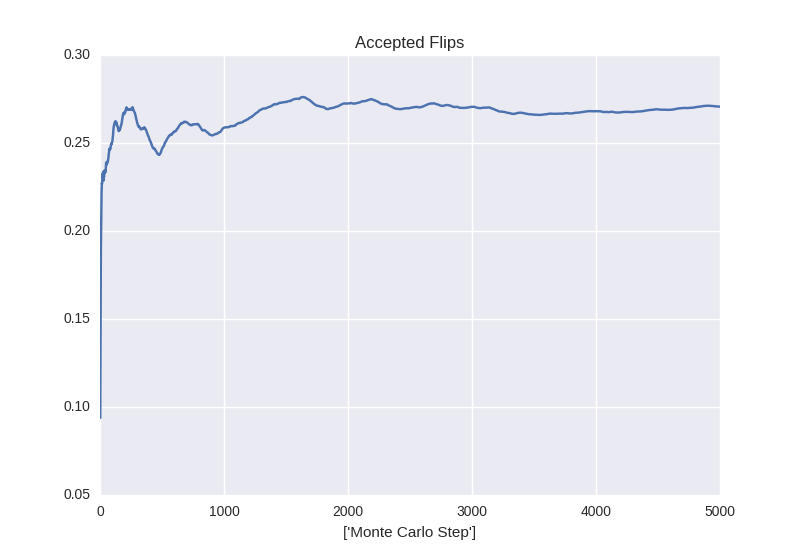
\includegraphics[height=2.2in]{flipsWUpStartT24.png}
        \caption{Mean absolute magnetic moment per spin from uniform start}
    \end{subfigure}
      \caption{Time development of mean energy and mean magic moment per spin for two different initial configurations.}\label{fig:20x20_Sweep_flips}
\end{figure}
All these figures seem to indicate that equilibrium is quickly reached (after less than 2000 cycles). However, sometimes this is not the case, as we hit a local minimum (described in more detail \textbf{HERE}). This gives the following plots:


\begin{figure}[!ht]
    \centering
    \begin{subfigure}[H!]{0.5\textwidth}
        \centering
        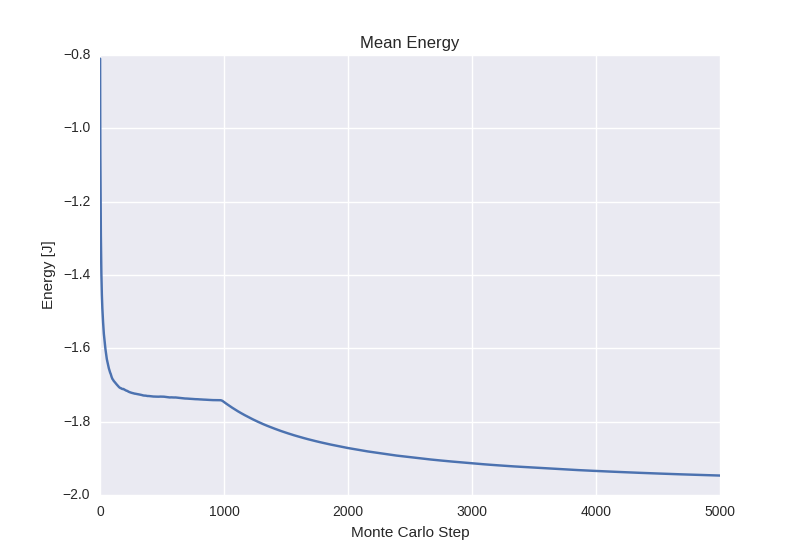
\includegraphics[height=2.2in]{meanEnergyLocalMin.png}
        \caption{Mean energy per spin from disordered state}
    \end{subfigure}%
    ~ 
    \begin{subfigure}[H!]{0.5\textwidth}
        \centering
        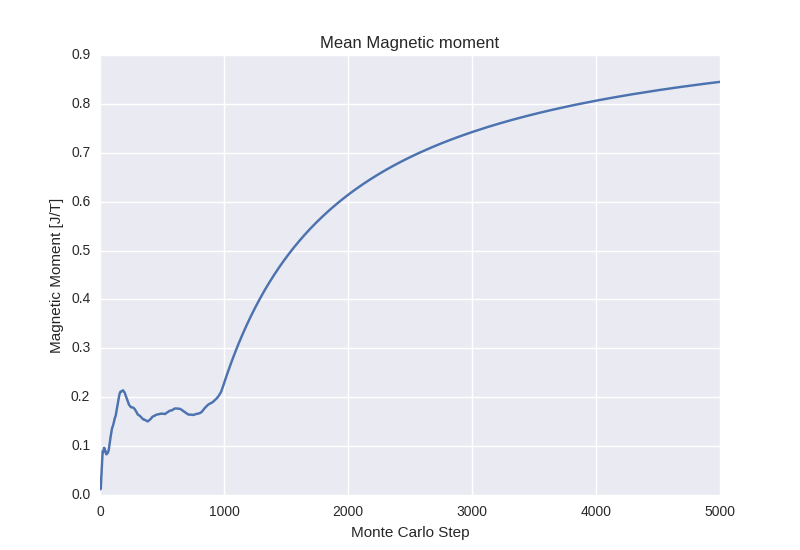
\includegraphics[height=2.2in]{meanMagMomLocalMin.png}
        \caption{Mean energy per spin from uniform state}
    \end{subfigure}
     ~ 
    \begin{subfigure}[H!]{0.5\textwidth}
        \centering
        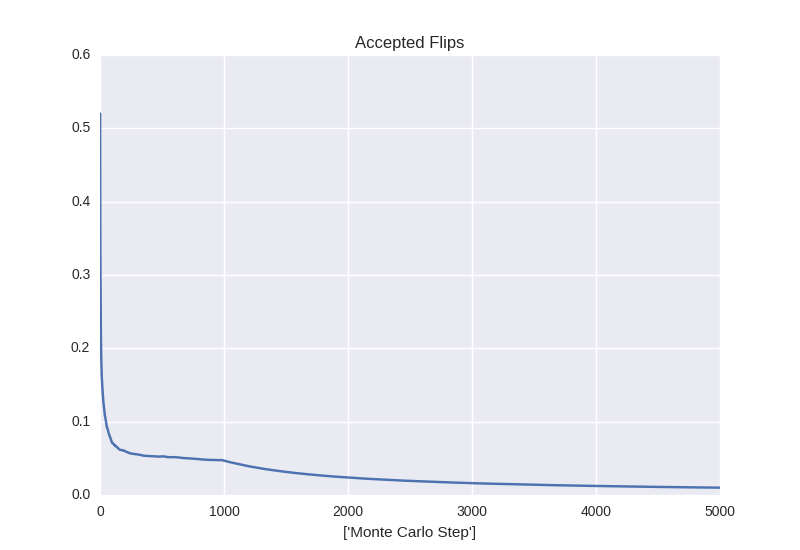
\includegraphics[height=2.2in]{flipsLocalMin.png}
        \caption{Mean energy per spin from uniform state}
    \end{subfigure}
       \caption{Time development of mean energy and mean magic moment per spin for two different initial configurations.}\label{fig:20x20_Sweep_flips}
\end{figure}
This shows that it sometimes takes significantly longer to arrive at equilibrium. Furthermore, equilibration time may also increase for higher temperature. Therefore, we choose 5000 Monte Carlo cycles as a safe equilibration time.
\subsection{Results from our investigation into the probability distribution}
Here we plot the probability of a certain energy occurring for two different temperatures. We plot this both as a curve and as a histogram.
\begin{figure}[!ht]
    \centering
    \begin{subfigure}[H!]{0.5\textwidth}
        \centering
        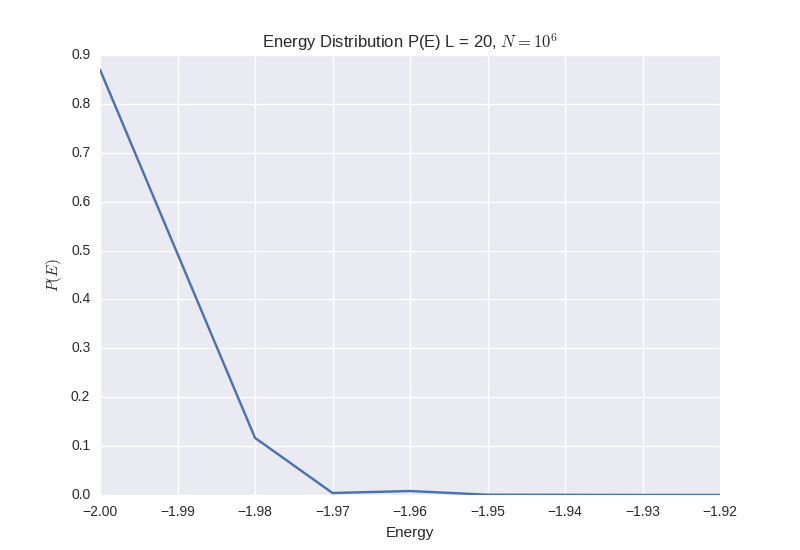
\includegraphics[height=2.2in]{energyDistT1.png}
        \caption{Mean energy per spin from disordered state}
    \end{subfigure}%
    ~ 
    \begin{subfigure}[H!]{0.5\textwidth}
        \centering
        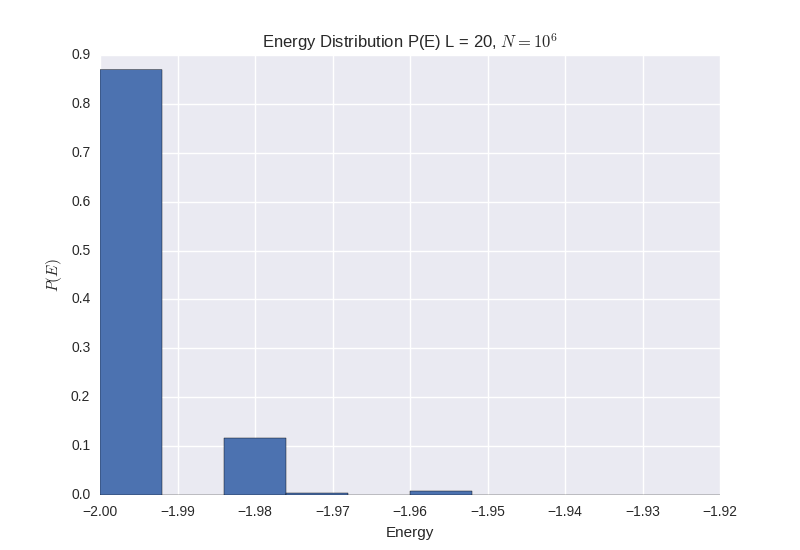
\includegraphics[height=2.2in]{energyDistHistoT1.png}
        \caption{Mean energy per spin from disordered state}
    \end{subfigure}
        ~
  \begin{subfigure}[H!]{0.5\textwidth}
        \centering
        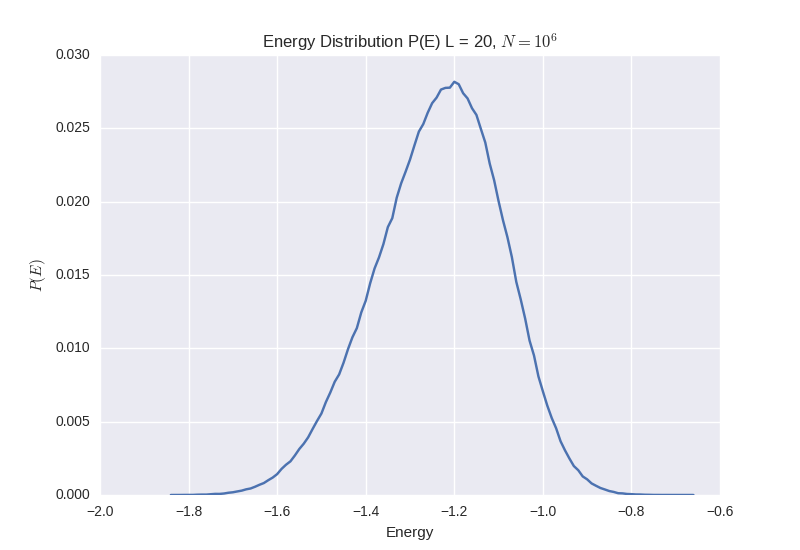
\includegraphics[height=2.2in]{energyDist.png}
        \caption{Mean energy per spin from uniform state}
   \end{subfigure}
         ~ 
  \begin{subfigure}[H!]{0.5\textwidth}
        \centering
        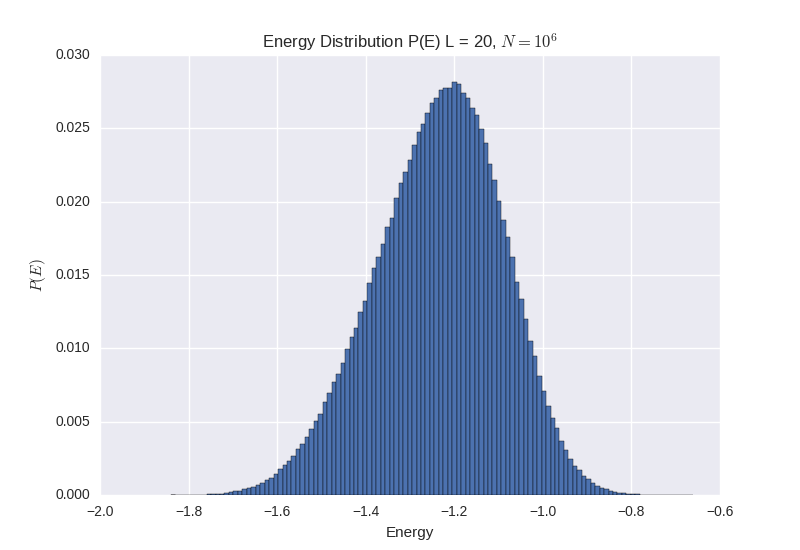
\includegraphics[height=2.2in]{energyDistHisto.png}
        \caption{Mean energy per spin from uniform state}
  \end{subfigure}
       \caption{Time development of mean energy and mean magic moment per spin for two different initial configurations.}
\end{figure}

\subsection{Results from our investigation of phase transitions}
Here, we wish to investigate how the critical temperature, which we extract by looking at the susceptibility and heat capacity, depends on our lattice size $L$. We also include the mean energy and the absolute value of the mean magnetization for completeness. 
\begin{figure}[!ht]
    \centering
    \begin{subfigure}[H!]{0.5\textwidth}
        \centering
        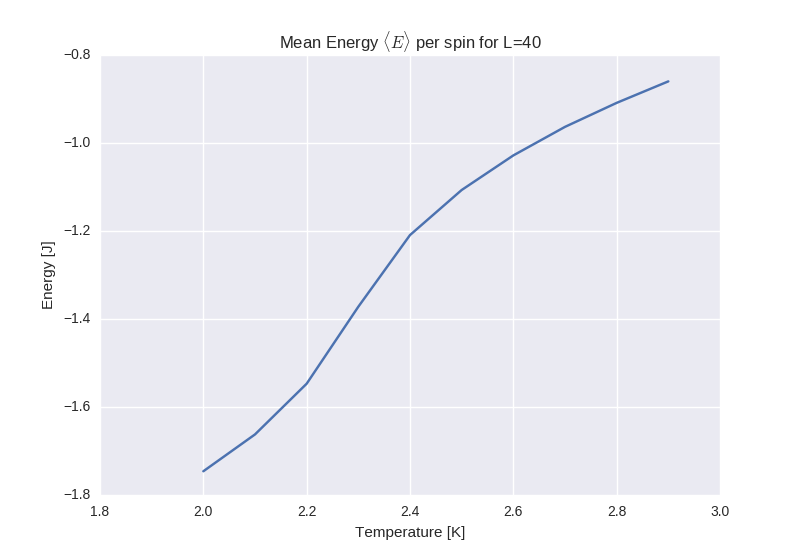
\includegraphics[height=2.2in]{meanEnergyl40Ne5.png}
        \caption{Mean energy per spin from disordered state}
    \end{subfigure}%
    ~ 
    \begin{subfigure}[H!]{0.5\textwidth}
        \centering
        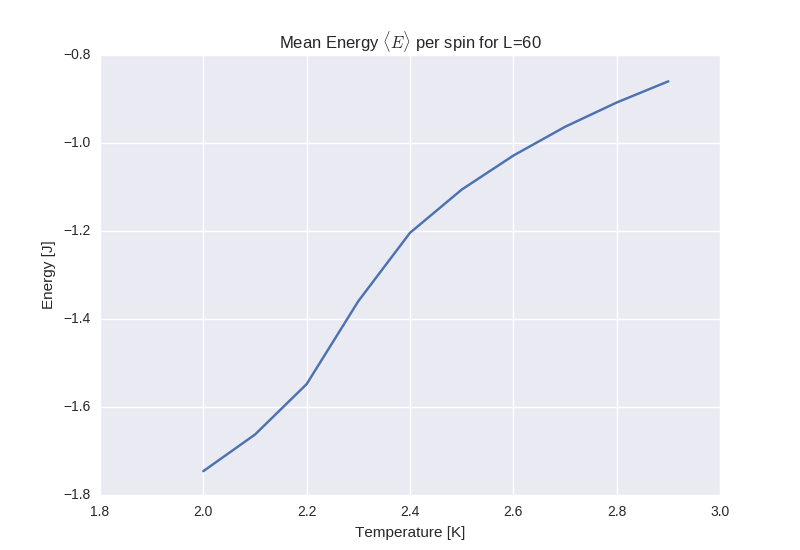
\includegraphics[height=2.2in]{meanEnergyl60Ne5.png}
        \caption{Mean energy per spin from uniform state}
    \end{subfigure}
        ~
     \begin{subfigure}[H!]{0.5\textwidth}
        \centering
        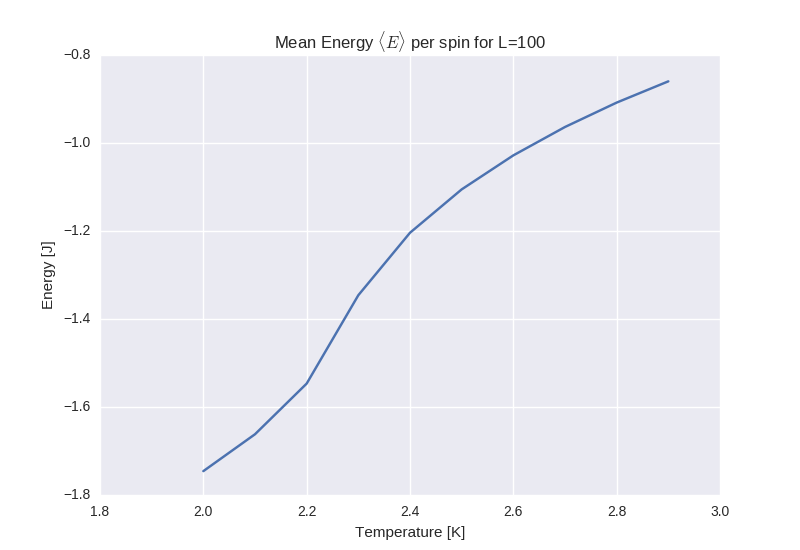
\includegraphics[height=2.2in]{meanEnergyl100Ne5.png}
        \caption{Mean absolute magnetic moment per spin from disordered state}
    \end{subfigure}%
    ~ 
    \begin{subfigure}[H!]{0.5\textwidth}
        \centering
        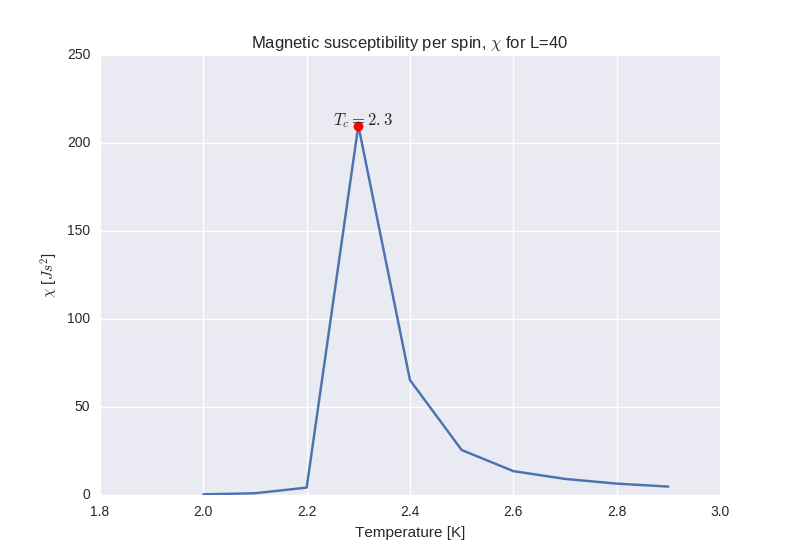
\includegraphics[height=2.2in]{chil40Ne5.png}
        \caption{Mean absolute magnetic moment per spin from uniform start}
    \end{subfigure}
      \caption{Time development of mean energy and mean magic moment per spin for two different initial configurations.}
\end{figure}
\begin{figure}[!ht]
    \centering
    \begin{subfigure}[H!]{0.5\textwidth}
        \centering
        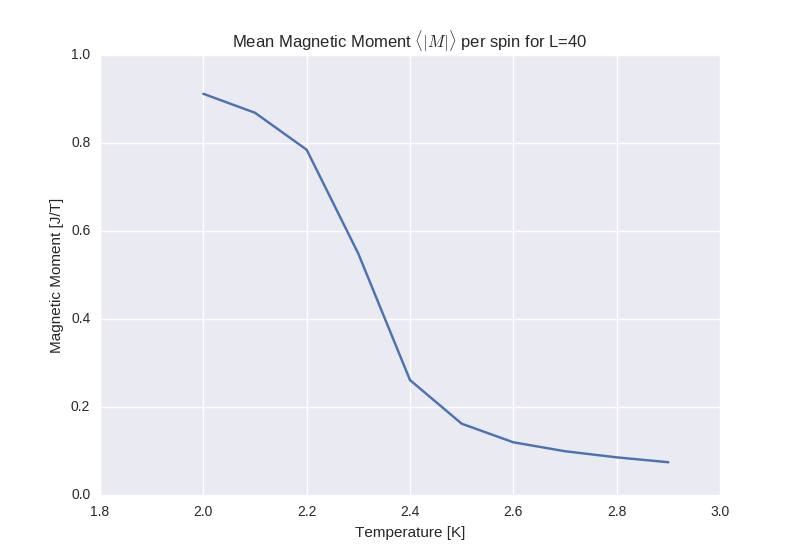
\includegraphics[height=2.2in]{meanMagMonl40Ne5.png}
        \caption{Mean energy per spin from disordered state}
    \end{subfigure}%
    ~ 
    \begin{subfigure}[H!]{0.5\textwidth}
        \centering
        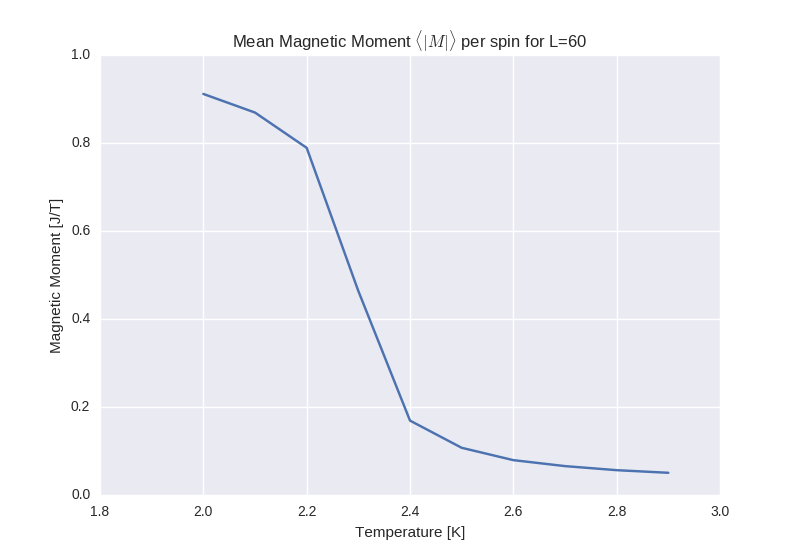
\includegraphics[height=2.2in]{meanMagMoml60Ne5.png}
        \caption{Mean energy per spin from uniform state}
    \end{subfigure}
        ~
     \begin{subfigure}[H!]{0.5\textwidth}
        \centering
        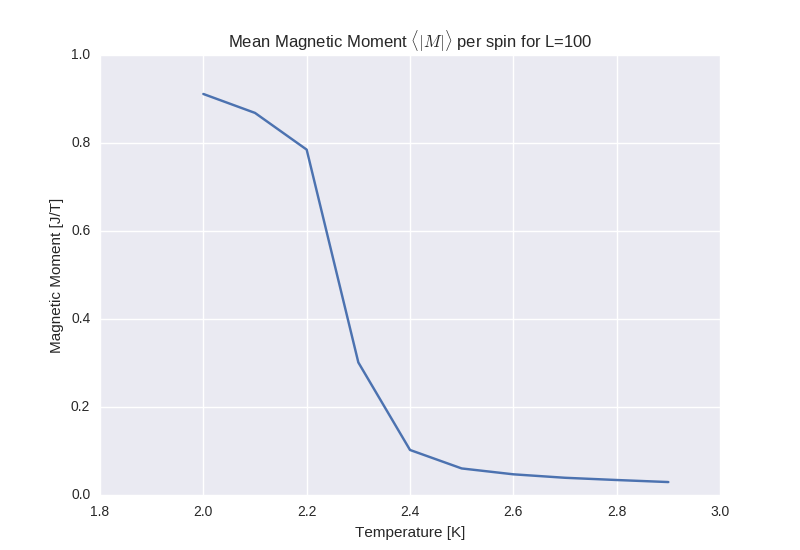
\includegraphics[height=2.2in]{meanMagMoml100Ne5.png}
        \caption{Mean absolute magnetic moment per spin from disordered state}
    \end{subfigure}%
    ~ 
    \begin{subfigure}[H!]{0.5\textwidth}
        \centering
        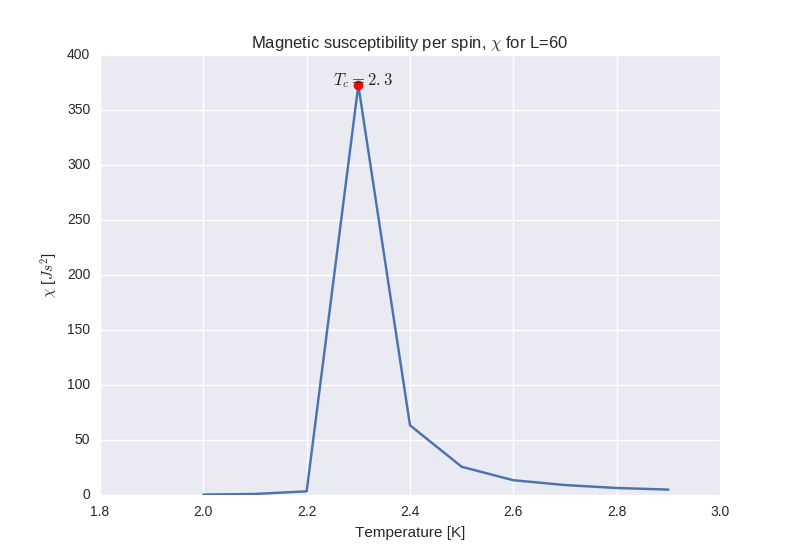
\includegraphics[height=2.2in]{chil60Ne5.png}
        \caption{Mean absolute magnetic moment per spin from uniform start}
    \end{subfigure}
      \caption{Time development of mean energy and mean magic moment per spin for two different initial configurations.}
\end{figure}
\begin{figure}[!ht]
    \centering
    \begin{subfigure}[H!]{0.5\textwidth}
        \centering
        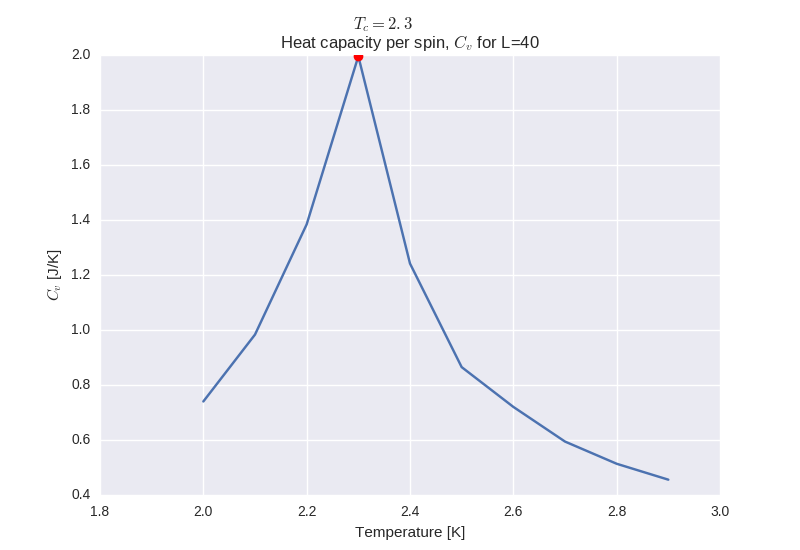
\includegraphics[height=2.2in]{cvl40Ne5.png}
        \caption{Mean energy per spin from disordered state}
    \end{subfigure}%
    ~ 
    \begin{subfigure}[H!]{0.5\textwidth}
        \centering
        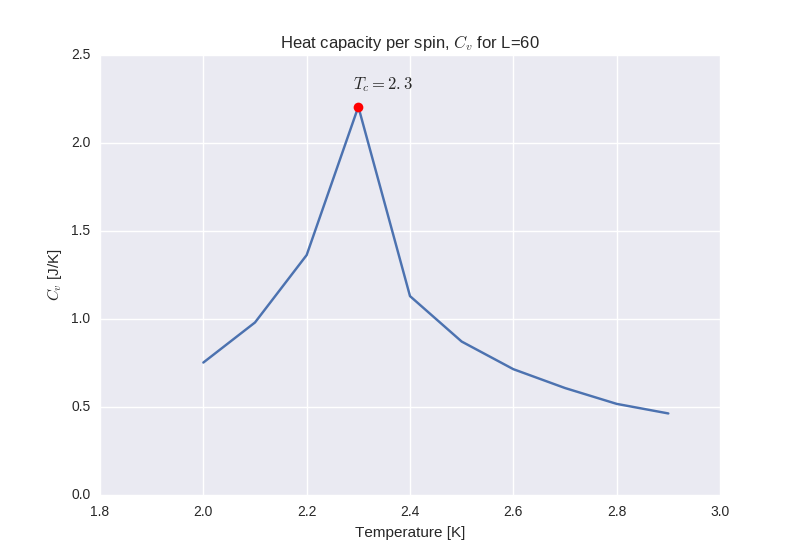
\includegraphics[height=2.2in]{cvl60Ne5.png}
        \caption{Mean energy per spin from uniform state}
    \end{subfigure}
        ~
     \begin{subfigure}[H!]{0.5\textwidth}
        \centering
        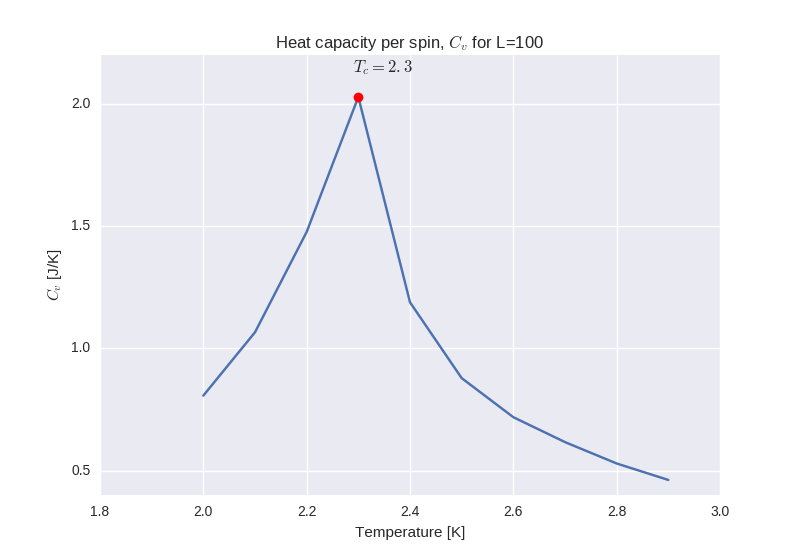
\includegraphics[height=2.2in]{cvl100Ne5.png}
        \caption{Mean absolute magnetic moment per spin from disordered state}
    \end{subfigure}%
    ~ 
    \begin{subfigure}[H!]{0.5\textwidth}
        \centering
        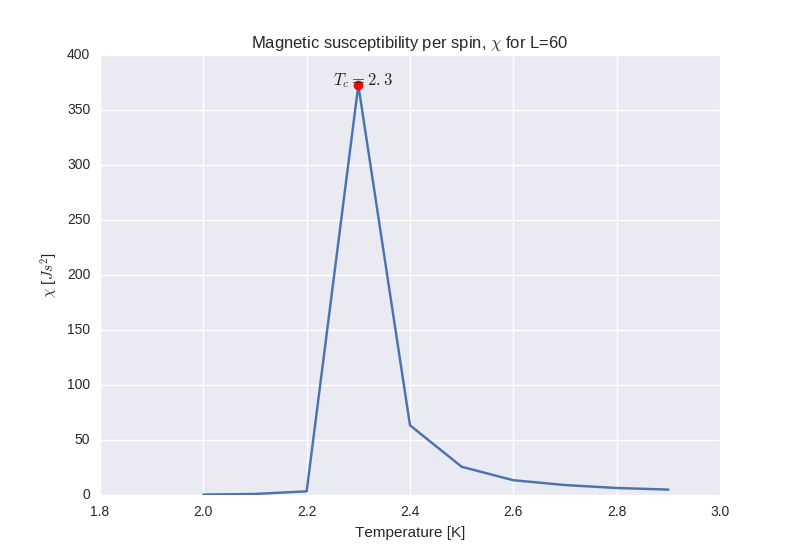
\includegraphics[height=2.2in]{chil60Ne5.png}
        \caption{Mean absolute magnetic moment per spin from uniform start}
    \end{subfigure}
      \caption{Time development of mean energy and mean magic moment per spin for two different initial configurations.}
\end{figure}
\begin{figure}[!ht]
    \centering
    \begin{subfigure}[H!]{0.5\textwidth}
        \centering
        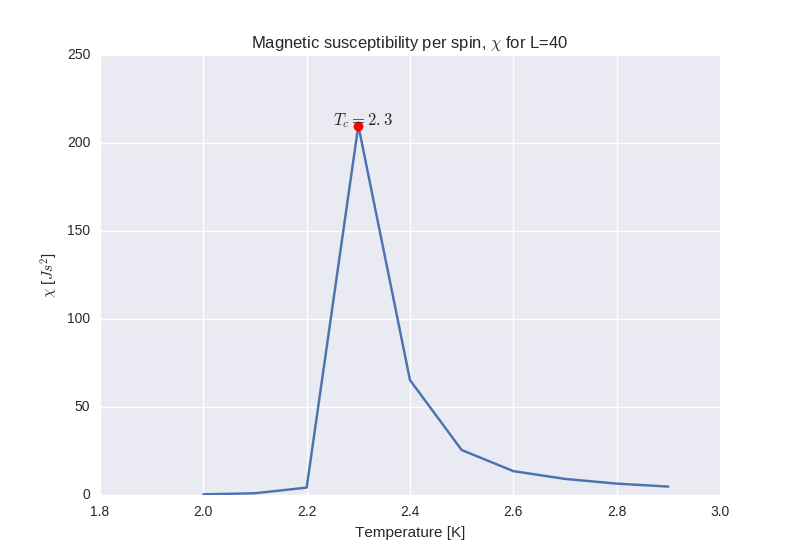
\includegraphics[height=2.2in]{chil40Ne5.png}
        \caption{Mean energy per spin from disordered state}
    \end{subfigure}%
    ~ 
    \begin{subfigure}[H!]{0.5\textwidth}
        \centering
        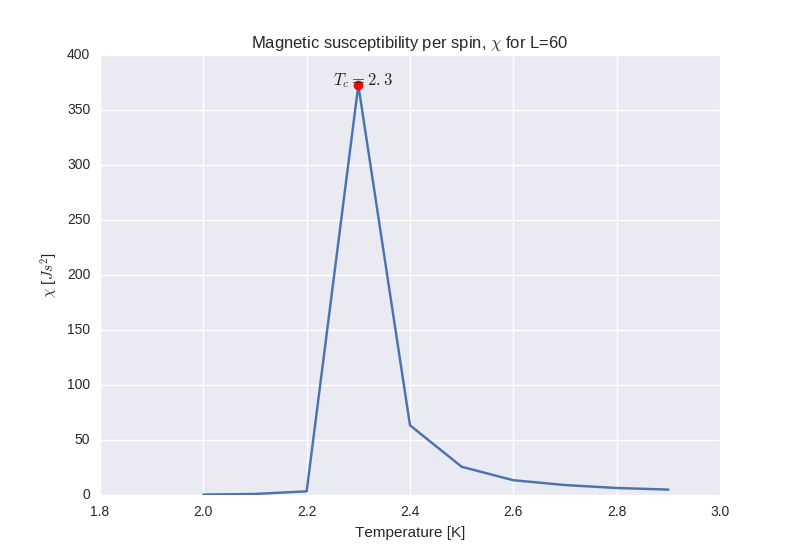
\includegraphics[height=2.2in]{chil60Ne5.png}
        \caption{Mean energy per spin from uniform state}
    \end{subfigure}
        ~
     \begin{subfigure}[H!]{0.5\textwidth}
        \centering
        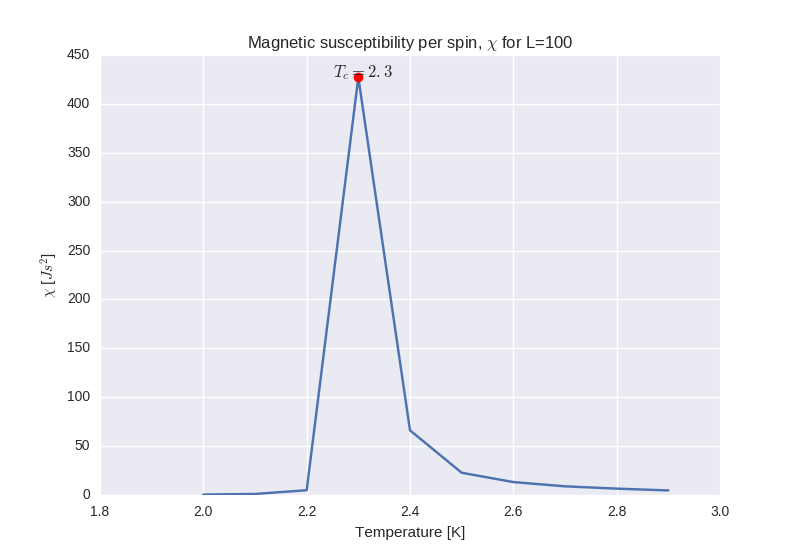
\includegraphics[height=2.2in]{chil100Ne5.png}
        \caption{Mean absolute magnetic moment per spin from disordered state}
    \end{subfigure}%
    ~ 
    \begin{subfigure}[H!]{0.5\textwidth}
        \centering
        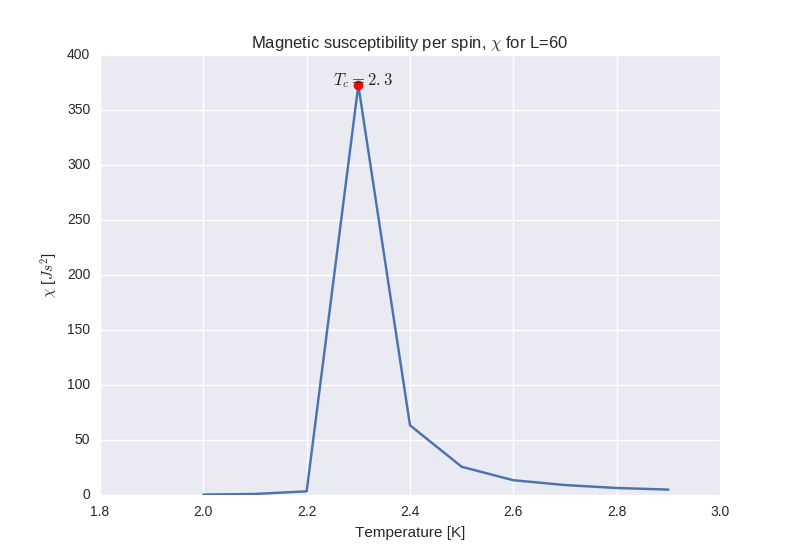
\includegraphics[height=2.2in]{chil60Ne5.png}
        \caption{Mean absolute magnetic moment per spin from uniform start}
    \end{subfigure}
      \caption{Time development of mean energy and mean magic moment per spin for two different initial configurations.}
\end{figure}
\subsection{Results from parallelizing our code}
\section{Discussion}
\subsection{The 2 $\times$ 2 lattice}
Figure \ref{fig:2x2_nsteps} compares the analytic and numeric solution for a different number of Monte Carlo cycles. As expected, our numeric solution approaches the analytic solution with increasing $N$, and for $N=4\times 10^7$, the solutions are barely distinguishable. Therefore, we adapt this as an acceptable $N$, for this system.  Note further that, with this $N$,all other thermodynamic quantities shown in figure \ref{fig:2x2_thermo} are also very well reproduced by our code. This shows that our simulations converge to the expected values for the $2\times2$ lattice, which hopefully implies that our code also works for larger lattices, for which there are no analytic solutions. Note, however, that $N=10^7$ was not attainable within our strict time constraints. Therefore, we performed the remaining simulations with $N=10^5$, but start the computation after equilibrium has  been reached.  
\section{Conclusion}
\end{document}

